\documentclass[
%draft,%
twoside,%
%openleft,%
%twocolumn,%
%titlepage,%
%fleqn,%
%a4page,%
ngerman,%
headsepline%
%a4paper,%
11pt]%
{article}

% Pakete
\usepackage{fancyhdr}
\usepackage{graphicx}
\usepackage[applemac]{inputenc}
%\usepackage{german}
\usepackage{../../../../../Documents/Mathematik/mymath}
\usepackage{units}
\usepackage{nicefrac}
\usepackage{pgf,tikz}
\usetikzlibrary{arrows}
\usepackage[T1]{fontenc}

%\usepackage{fancyhdr}
%\usepackage{scrpage2}
\usepackage{lastpage}
\usepackage{geometry}
\usepackage{graphicx}
\usepackage[applemac]{inputenc}
\usepackage[ngerman]{babel}
\usepackage{lscape}
%\usepackage{/Users/waj/Documents/Mathematik/mymath}
%\usepackage{units}
%\usepackage{nicefrac}
%\usepackage{pgf,tikz}
%\usetikzlibrary{arrows}
\usepackage{colortbl}
\usepackage{hhline}
\usepackage{multirow}
\usepackage[extendedchars]{grffile}
\usepackage{caption}
\usepackage{multicol,calc}
\usepackage{blindtext}
\usepackage{pdfpages}
\usepackage{hyperref}
\usepackage{wrapfig}

% Seite auf A4-Format anpassen
%\setlength{\textheight}{650pt}%
%\setlength{\voffset}{-45pt}%
%\setlength{\textwidth}{444pt}%
%\setlength{\hoffset}{-41pt}%

%Setting margins to open right my script
\let\tmp\oddsidemargin
\let\oddsidemargin\evensidemargin
\let\evensidemargin\tmp
\reversemarginpar

% Header und Footer
\pagestyle{fancy}
\fancypagestyle{myheadings}{%
\renewcommand{\footrulewidth}{0pt}
\headheight 50pt

\rhead{\hrule \ \\[1ex]
\begin{minipage}[b]{26ex}
Angewandte Mathematik\\
Differenzialgleichungen\\
Raketengleichung\\
gymkl, WaJ\\[-2.5ex]
\end{minipage}
}

\chead{}%
\lhead{\Huge \textbf{\textsc{Raketengleichung}}\\[-1ex]}%
\rfoot{}%
\cfoot{\thepage}%
\lfoot{}%
}

\fancypagestyle{plain}{%
\headheight 30pt
\renewcommand{\headrulewidth}{0pt}
\renewcommand{\footrulewidth}{0pt}
\rhead{}%
\chead{}%
\lhead{}%
\rfoot{}%
\cfoot{}%
\lfoot{}%
}


\begin{document}
\pagestyle{myheadings}

\section{Modell}
\begin{figure}
  \begin{center}
    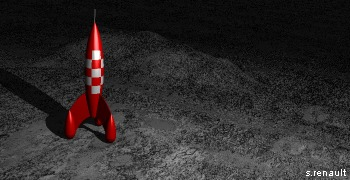
\includegraphics[width=0.618\textwidth]{pictures/raketetim}
  \end{center}
%\caption{A gull}
\end{figure}

Wir betrachten das klassische \glqq Pfupfmodel\grqq\ einer Rakete der Masse $m$ mit Geschwindigkeit $v$ und verwenden den Impulserhaltungssatz. Also notieren wir jeweils den Impuls $p$ vor und nach dem \glqq Stoss\grqq\ und vergleichen.

\begin{figure}[h!]
  \begin{center}
    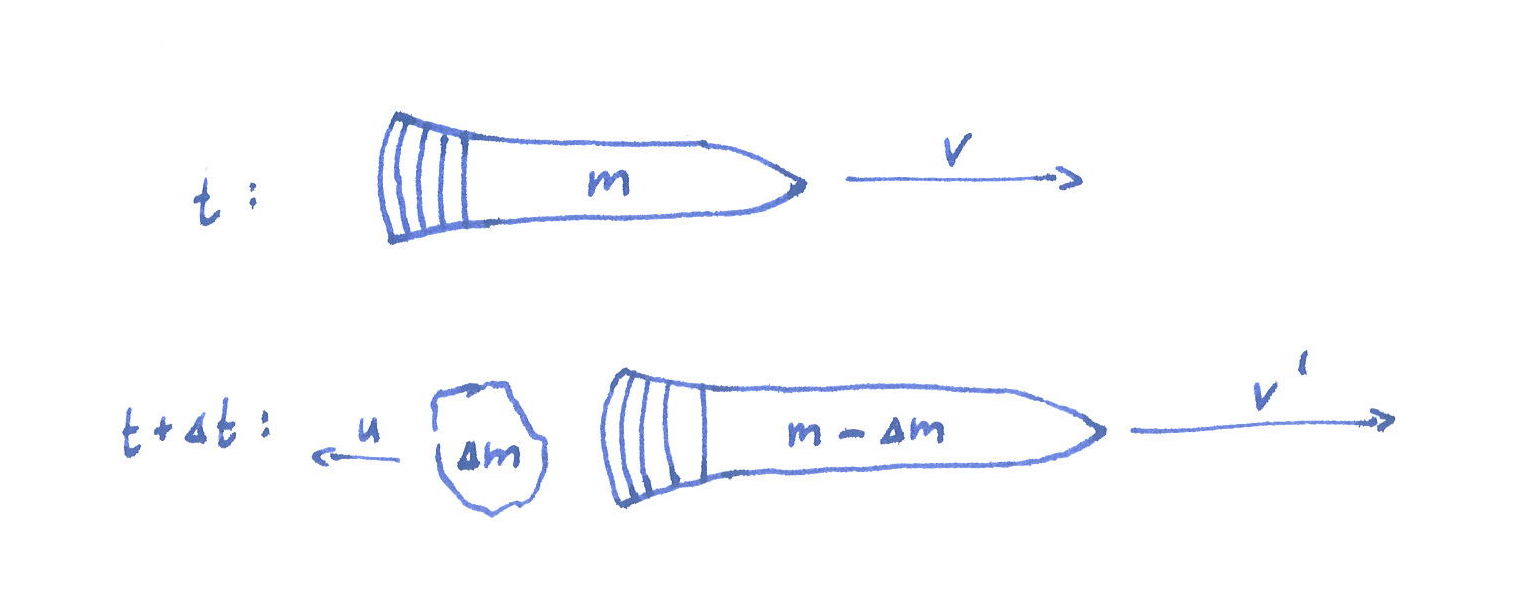
\includegraphics[width=0.618\textwidth]{pictures/raketeimpuls}
  \end{center}
%\caption{A gull}
\end{figure}

Mit obiger Notation gilt:
$$p=(m-\gD m)\cdot v'+\gD m\cdot(v'-u)$$
und unmittelbar folgt f�r $p=mv$
$$mv=mv'-\gD mu$$
wobei $v'$ die Geschwindigkeit der Rakete nach dem Stoss und $u$ die Ausstr�mgeschwindigkeit des Gases bezeichnet.

Davon hat man noch nicht viel. Berechnen wir vielleicht die Geschwindigkeit bzw. den Geschwindigkeitsverlauf der Rakete. Wir l�sen
$$mv=mv'-\gD mu$$
nach $v'-v$ und bezeichnen diese Differenz mit $\gD v$; explizit
$$\gD v=\frac{\gD mu}{m}.$$
F�r $\gD t\to0$ erhalten wir die Differentialgleichung
$$dv=-\frac{dm}{m}\cdot u.$$
�ber das Vorzeichen l�sst sich streiten; anyway. Wir integrieren, um die Geschwindigkeit zu erhalten:
$$\int_{v_0}^v\,dv=\int_{m_0}^m-\frac{u}{m}\,dm.$$
Also gilt f�r die Geschwindigkeit der Rakete mit Anfangsmasse $m_0$ und Anfangsgeschwindigkeit $v_0$
$$v(t)=v_0+u\cdot\ln\left(\frac{m_0}{m}\right).$$
Dieser Ausdruck wird auch {\bf 1. Raketengleichung} genannt. Sie gibt die Geschwindigkeit einer Rakete im Vakuum ohne Gravitationseinfluss an.

\section{Analyse}
\subsection{Geschwindigkeitsverlauf}

Wir zeichnen vorerst das $v$-$t$-Diagramm. Dazu m�ssen wir beachten, dass $m$ auch von der Zeit abh�ngt, $m=m(t)$.
$$v(t)=v_0+u\cdot\ln\left(\frac{m_0}{m(t)}\right).$$
Nehmen wir einen zeitlich konstanten Gasausstoss $\gm$ an, so gilt f�r die Masse der Rakete zur Zeit $t$
$$m(t)=m_0-\gm t$$
und damit f�r die Geschwindigkeit
$$v(t)=v_0+u\cdot\ln\left(\frac{m_0}{m_0-\gm t}\right).$$

So, setzen wir $v_0=0$, $u=2500$, $m_0=2200$ und $\gm=2.5$ und schauen uns Abbildung \ref{geschwindigkeitrakete} an.

\begin{figure}
\definecolor{cqcqcq}{rgb}{0.752941176471,0.752941176471,0.752941176471}
\begin{center}
\begin{tikzpicture}[line cap=round,line join=round,>=triangle 45,x=0.01cm,y=0.00065cm]
\draw [color=cqcqcq,dash pattern=on 3pt off 3pt, xstep=1.0cm,ystep=1.31cm] (0,0) grid (900.,9900);
\draw[->,color=black] (-100.,0.) -- (900.,0.);
\foreach \x in {100,200,300,400,500,600,700,800}
\draw[shift={(\x,0)},color=black] (0pt,2pt) -- (0pt,-2pt) node[below] {\footnotesize $\x$};
\draw[color=black] (872.413793103,89.172) node [anchor=south west] { t};
\draw[->,color=black] (0.,-100.) -- (0.,10000.0028571);
\foreach \y in {2000,4000,6000,8000}
\draw[shift={(0,\y)},color=black] (2pt,0pt) -- (-2pt,0pt) node[left] {\footnotesize $\y$};
\draw[color=black] (8.62068965517,9509.55685714) node [anchor=west] { v(t)};
\clip(-100.,-500.000142857) rectangle (900.,10000.0028571);
\draw[line width=1.2pt,smooth,samples=100,domain=0:865.0000000000001] plot(\x,{2500.0*ln(2200.0/(2200.0-2.5*(\x)))});
\begin{scriptsize}
\end{scriptsize}
\end{tikzpicture}
\end{center}
\caption{Geschwindigkeitsverlauf der Rakete}\label{geschwindigkeitrakete}
\end{figure}


Man sieht, dass die Rakete immer st�rker beschleunigt. So lange, bis der Brennstoff aufgebraucht ist. Wie lange dauert das? Um diese Frage zu beantworten, nehmen wir uns $m_0$ vor und schreiben
$$m_0=m_{leer}+m_{brenn}.$$
Dabei ist nat�rlich zu beachten, dass $m_{leer}$ inklusive Nutzlast aufzufassen ist. Ist zum Beispiel $m_{leer}=200$, so erh�lt man f�r $m_{brenn}=\gm\cdot t_{brenn}$ die Brenndauer
$$t_{brenn}=\frac{m_{brenn}}{\gm}.$$
F�r obige Werte hat man $t_{brenn}=\unit[800]{Sekunden}$.

\subsection{Brennschlussgeschwindigkeit}

Von Interesse ist auch, welche Endgeschwindigkeit die Rakete erreicht. Wir setzen also im Geschwindigkeitsverlauf $m_0=m_{leer}$, da ja kein Brennstoff mehr vorhanden ist. Numerisch ergibt sich
$$v_e=v_0+u\cdot\ln\left(\frac{m_0}{m_{leer}}\right)\approx\unitfrac[6000]{m}{s}$$

Man will die Endgeschwindigkeit optimieren. Sie ist proportional zur Ausstr�mgeschwindigkeit und h�ngt logarithmisch vom Verh�ltnis Masse beim Start zu Masse nach Brennschluss ab. Mehr Erkenntnis gibt unser Model nicht her.

\subsection{Nutzlasten}

Will man Material in eine Umlaufbahn bringen, so muss man grosse Endgeschwindigkeiten erreichen k�nnen. Wir betrachten, wiederum f�r $v_0=0$, das Verh�ltnis von Endgeschwindigkeit zu Gasgeschwindigkeit:
$$\frac{v_e}{u}=\ln\left(\frac{m_0}{m_{leer}}\right)=\ln\left(1+\frac{m_{brenn}}{m_{leer}}\right).$$
Also ist der Zusammenhang vom Typ
$$v_v=\ln(1+m_v)$$
mit $v_v=\frac{v_e}{u}$ und $m_v=\frac{m_{brenn}}{m_{leer}}$ oder in der Anschauung in Abbildung \ref{raketeverhaeltnis}.

\begin{figure}
\definecolor{cqcqcq}{rgb}{0.752941176471,0.752941176471,0.752941176471}
\begin{center}
\begin{tikzpicture}[line cap=round,line join=round,>=triangle 45,x=0.15cm,y=1.2cm]
\draw [color=cqcqcq,dash pattern=on 2pt off 2pt, xstep=1.5cm,ystep=1.2cm] (0,0) grid (65.7327586207,4.8);
\draw[->,color=black] (-5.,0.) -- (65.7327586207,0.);
\foreach \x in {10,20,30,40,50,60}
\draw[shift={(\x,0)},color=black] (0pt,2pt) -- (0pt,-2pt) node[below] {\footnotesize $\x$};
\draw[color=black] (63.0172413793,0.0509554140127) node [anchor=south west] { $m_v$};
\draw[->,color=black] (0.,-0.5) -- (0.,5.);
\foreach \y in {1,2,3,4}
\draw[shift={(0,\y)},color=black] (2pt,0pt) -- (-2pt,0pt) node[left] {\footnotesize $\y$};
\draw[color=black] (0.646551724138,4.65605095541) node [anchor=west] { $v_v$};
\draw[color=black] (0pt,-10pt) node[right] {\footnotesize $0$};
\clip(-5.,-0.859872611465) rectangle (65.7327586207,5.);
\draw[smooth,samples=100,domain=0.00001:65.73275862068971] plot(\x,{ln(1.0+(\x))});
\begin{scriptsize}
\end{scriptsize}
\end{tikzpicture}
\end{center}
\caption{Verh�ltnisgleichung}\label{raketeverhaeltnis}
\end{figure}

Selbst bei einem Verh�ltnis von $50$ von Brennstoff zu Leermasse erh�lt man nur eine $4$mal so grosse Endgeschwindigkeit wie die Ausstr�mgeschwindigkeit.

\begin{bem}
Es ist problematisch, grosse Nutzlasten auf hohe Endgeschwindigkeiten zu bringen.
\end{bem}

Folgend einige Werte von Ausstr�mgeschwindigkeiten, die heute erreicht werden k�nnen:
\begin{description}
\item[Feststoffrakete] $\unitfrac[2000]{m}{s}$
\item[Fl�ssigbrennstoffrakete] $\unitfrac[3200]{m}{s}$
\item[Hybride] $\unitfrac[4000]{m}{s}$
\end{description}

Nun, welche Geschwindigkeit muss eine Rakete erreichen, um das Gravitationsfeld der Erde zu verlassen --- die sogenannte Fluchtgeschwindigkeit? Mit Energieerhaltung
$$G\cdot\frac{Mm}{r}=\frac{1}{2}mv_2^2$$
erh�lt man
$$v_2=\sqrt{\frac{2GM}{r}}.$$
Um den Einflussbereich der Erde zu verlassen, muss eine Rakete eine Geschwindigkeit von $\unitfrac[11.2]{km}{s}$ erreichen.

\begin{bem}
Die konstruktive Obergrenze f�r eine einstufige Rakete liegt bei $15\div1$, womit klar ist, dass man mit einer einstufigen Rakete die Fluchtgeschwindigkeit (auch 2. kosmische Geschwindigkeit) nicht erreichen kann.
\end{bem}

\subsection{Rakete unter Schwerkrafteinfluss (g sonst)}

F�r einen senkrechten Wurf nach oben gilt
$$v(t)=v_0-gt$$
und somit f�r die Rakete
$$v(t)=u\cdot\ln\left(\frac{m_0}{m_0-\gm t}\right)-gt.$$
Mit den Werten $u=1000$, $m_0=1100$, $\gm=10$, $g=9.81$ berechnen wir noch die Brenndauer $t'$ via
$$m_{brenn}=\gm t'$$
und finden $t'=100$.
Nach Brennschluss haben wir
$$v(t)=v_{brenn}-gt$$
wobei $v_{brenn}$ die Brennschlussgeschwindigkeit bezeichnet. Da dieser Geschwindigkeitsverlauf erst nach Brennschluss stattfindet, verschieben wir die Funktion um die Zeit $t'$
$$v_{nach}(t)=v(t')-g(t-t')$$
Insgesamt haben wir
$$\tilde{v}(t)=
\begin{cases}
v(t)& t<t'\\
v_{nach}(t)& t\geq t'
\end{cases}
$$
Der Graph sieht folgendermassen aus:

\begin{figure}[h!]
\definecolor{cqcqcq}{rgb}{0.752941176471,0.752941176471,0.752941176471}
\begin{center}
\begin{tikzpicture}[line cap=round,line join=round,>=triangle 45,x=0.03cm,y=0.003cm]
\draw [color=cqcqcq,dash pattern=on 2pt off 2pt, xstep=1.5cm,ystep=0.6cm] (0,0) grid (300,1900);
\draw[->,color=black] (-30.,0.) -- (300.,0.);
\foreach \x in {50,100,150,200,250}
\draw[shift={(\x,0)},color=black] (0pt,2pt) -- (0pt,-2pt) node[below] {\footnotesize $\x$};
\draw[color=black] (290.896551724,18.6836668966) node [anchor=south west] { t};
\draw[->,color=black] (0.,-30.) -- (0.,2000.00148915);
\foreach \y in {200,400,600,800,1000,1200,1400,1600,1800}
\draw[shift={(0,\y)},color=black] (2pt,0pt) -- (-2pt,0pt) node[left] {\footnotesize $\y$};
\draw[color=black] (2.84482758621,1897.24132122) node [anchor=west] { v(t)};
\draw[color=black] (0pt,-10pt) node[right] {\footnotesize $0$};
\clip(-30.,-200.000287915) rectangle (300.,2000.00148915);
\draw[line width=1.2pt,smooth,samples=100,domain=0:100] plot(\x,{1000.0*ln(1100.0/(1100.0-10.0*(\x)))-9.81*(\x)});
\draw[smooth,samples=100,domain=100:244.444] plot(\x,{2398.0-9.81*(\x)});
\begin{scriptsize}
\end{scriptsize}
\end{tikzpicture}
\end{center}
\end{figure}

Wie hoch steigt bei diesem Geschwindigkeitsverlauf die Rakete? Wir bestimmen den Steigungsverlauf als Integral �ber den Geschwindigkeitsverlauf:
$$s(t)=\int_0^t\tilde{v}(\gt)\,d\gt.$$
Vor Brennschluss haben wir
$$s(t)=\int \left[u\cdot\ln\left(\frac{m_0}{m_0-\gm t}\right)-gt\right]\,dt$$
und danach
$$s(t)=\int \left[v(t')-g(t-t')\right]\,dt.$$
Kompakt formuliert

$$\tilde{s}(t)=
\begin{cases}
-\frac{g}{2}t^2+ut+u(t-\frac{m_0}{\gm})\cdot\ln\left(\frac{m_0}{m_0-\gm t}\right)& t<t'\\
-\frac{g}{2}t^2+(gt'+v(t'))t& t\geq t'
\end{cases}
$$

\begin{bem}
Ein paar Dinge gefallen mir an diesem Model nicht.
\end{bem}

\end{document}